% vim: spelllang=en spell textwidth=120
\documentclass[deska]{subfiles}

\begin{document}

\chapter{A Gentle Introduction}

\begin{abstract}
The first chapter explains what Deska is, and what it tries to achieve.
\end{abstract}

\section{Motivation}

The Deska started as an internal project at the Institute of Physics of the~AS~CR,~v.v.i.~\cite{fzu}, out of a desire to make the
everyday operation of the regional grid computing centre smoother and reduce the set of tedious tasks that the staffers
had to perform during their regular maintenance.

One of the issues which the administrators at the Institute were fighting with was a high level of {\em duplicated
information}.  The data about machines in the server room were not available from a central place, but instead got
spread out into configuration files of many services and in-house databases.  Bind, the DNS daemon, provided mapping
between the DNS names and IP addresses, the configuration of the DHCP server listed pairs of the Ethernet MAC addresses
and IP addresses, names of switch ports were assigned by hand.  Various monitoring services had to include low-level
hardware information like the available disk size in order to be able to warn when the space begun to run out.  Roles of
machines, i.e. the desired purpose of each server, was mentioned in Cfengine's~\cite{cfengine} configuration, in the
Nagios~\cite{nagios} database and in many other places.  Adding new machines, retiring the old ones or even just
performing basic queries led to a rather tedious process where people had to consult each of the individual data sources
by hand and retrieve the desired piece of information.  Needless to say, this complicated workflow often led to working
with stale data or time wasted when troubleshooting an outdated network daemon configuration, and --- in the end ---
administrators who were unhappy with the process.

It was therefore decided that the Institute shall find a tool that can store all the information about the whole data
center, from hardware configuration and rack layout to network topology and provided application services, at a single,
authoritative place, and have a mechanism to {\em push} this data to various places which make use of it.  The Deska
project~\cite{deska-project} was formed to evaluate various existing tools which were available on the market in late
2009 and propose a system which would fit this goal.

Before we begun the initial design of the Deska project, we had evaluated various existing tools which were available
on the market at that time (see \secref{sec:evaluating-existing-tools} for details).  We came to the conclusion that
there is a market opportunity for a tool which --- instead of trying to reinvent the wheel --- works in close
collaboration with the existing infrastructure and serves as a glue layer between the individual services.

\section{The Deska Design}

The ultimate goal of Deska is to provide a central place for storing all information about the infrastructure of a
typical grid computing center, and subsequently {\em use} this central place to configure each and every device in the
network.

The Deska system is therefore built around a central object database.  When new data are pushed to the database by an
administrator, a set of hook scripts is run.  These scripts walk the objects in the database and produce configuration
files for each daemon and service.  The resulting configuration is then presented to the administrator who initiated the
change.  She can assess the difference in the generated configuration, decide whether it matches the changes she has made
to the database, and if she is happy with the result, approve the resulting configuration and new version of the
database data.  When approved, the system pushes the generated configuration files to the existing infrastructure for
fabric management, which takes care of distributing the updated data to the individual services.

\begin{figure}[h]
    \centering
    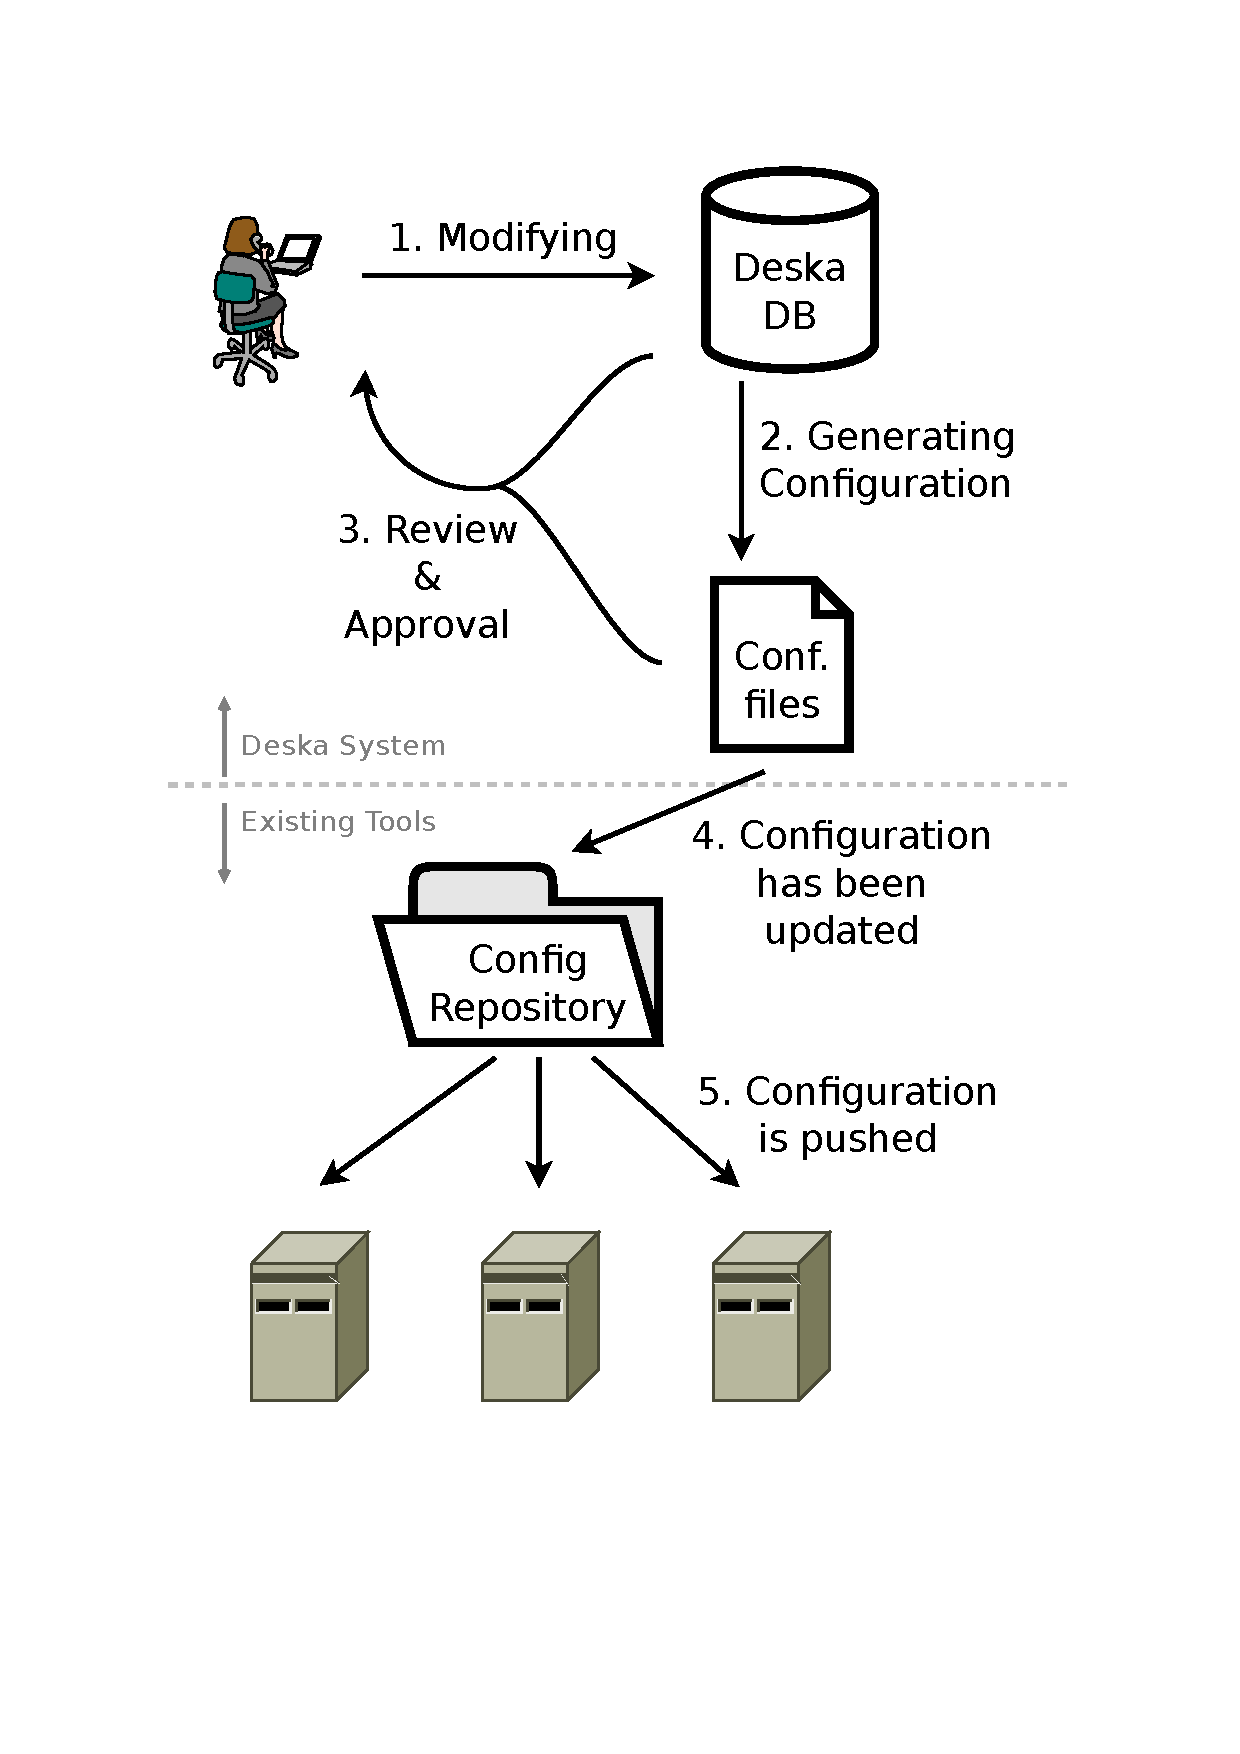
\includegraphics[trim=28mm 33mm 30mm 28mm, clip=true, width=75mm]{img-deska-workflow.pdf}
    \caption{Deska Workflow}
\end{figure}

In contrast to many existing tools, the Deska database scheme is not set in stone.  Experience at various sites
throughout the WLCG~\cite{wlcg} shows that each site prefers to stick with their own particular workflow.  Therefore, if
the Deska database imposed a fixed database layout, it would face rather strong opposition when pushed for adoption.  We
acknowledge that this is a political problem, not a technical one, but we have nonetheless chosen to design Deska as a
{\em generic} database.  Most of the code which ships with Deska is agnostic to the database layout the administrators
choose to use.  It is expected that installations of Deska at individual sites will differ only in the DB scheme and the
set of hook scripts which is used for configuration generators.

Nevertheless, it is clear that Deska cannot support a completely arbitrary database layout and at the same time provide
efficient client-side tools, which is why we impose some limits on the table structures.  These constraints are
explained in detail in~\secref{sec:objects-and-relations}.  A conforming database scheme is then fed to the Deska
installer, a tool which checks the scheme for validity and generates server-side SQL code.  This code provides full
support for data versioning, audit logging, constraint checking and many more server-side operations.

\section{Implementation}

The Deska system, as delivered, can be divided into four parts.  The first part, which is the most visible to the actual
user, is the CLI console, a text-mode application that connects to the Deska server and is intended to be used for
day-to-day work, from modifying the database to simple reporting.  The CLI console is implemented in C++ with heavy use
of the Boost libraries and is capable of discovering the database scheme on the fly, without any code changes.  It talks
to the Deska server over an SSH connection, using traditional Unix methods for authentication and authorization, through
a domain-specific JSON-based wire protocol (the Deska DBAPI, as described in~\secref{sec:dbapi-protocol}).

\begin{figure}[h]
    \centering
    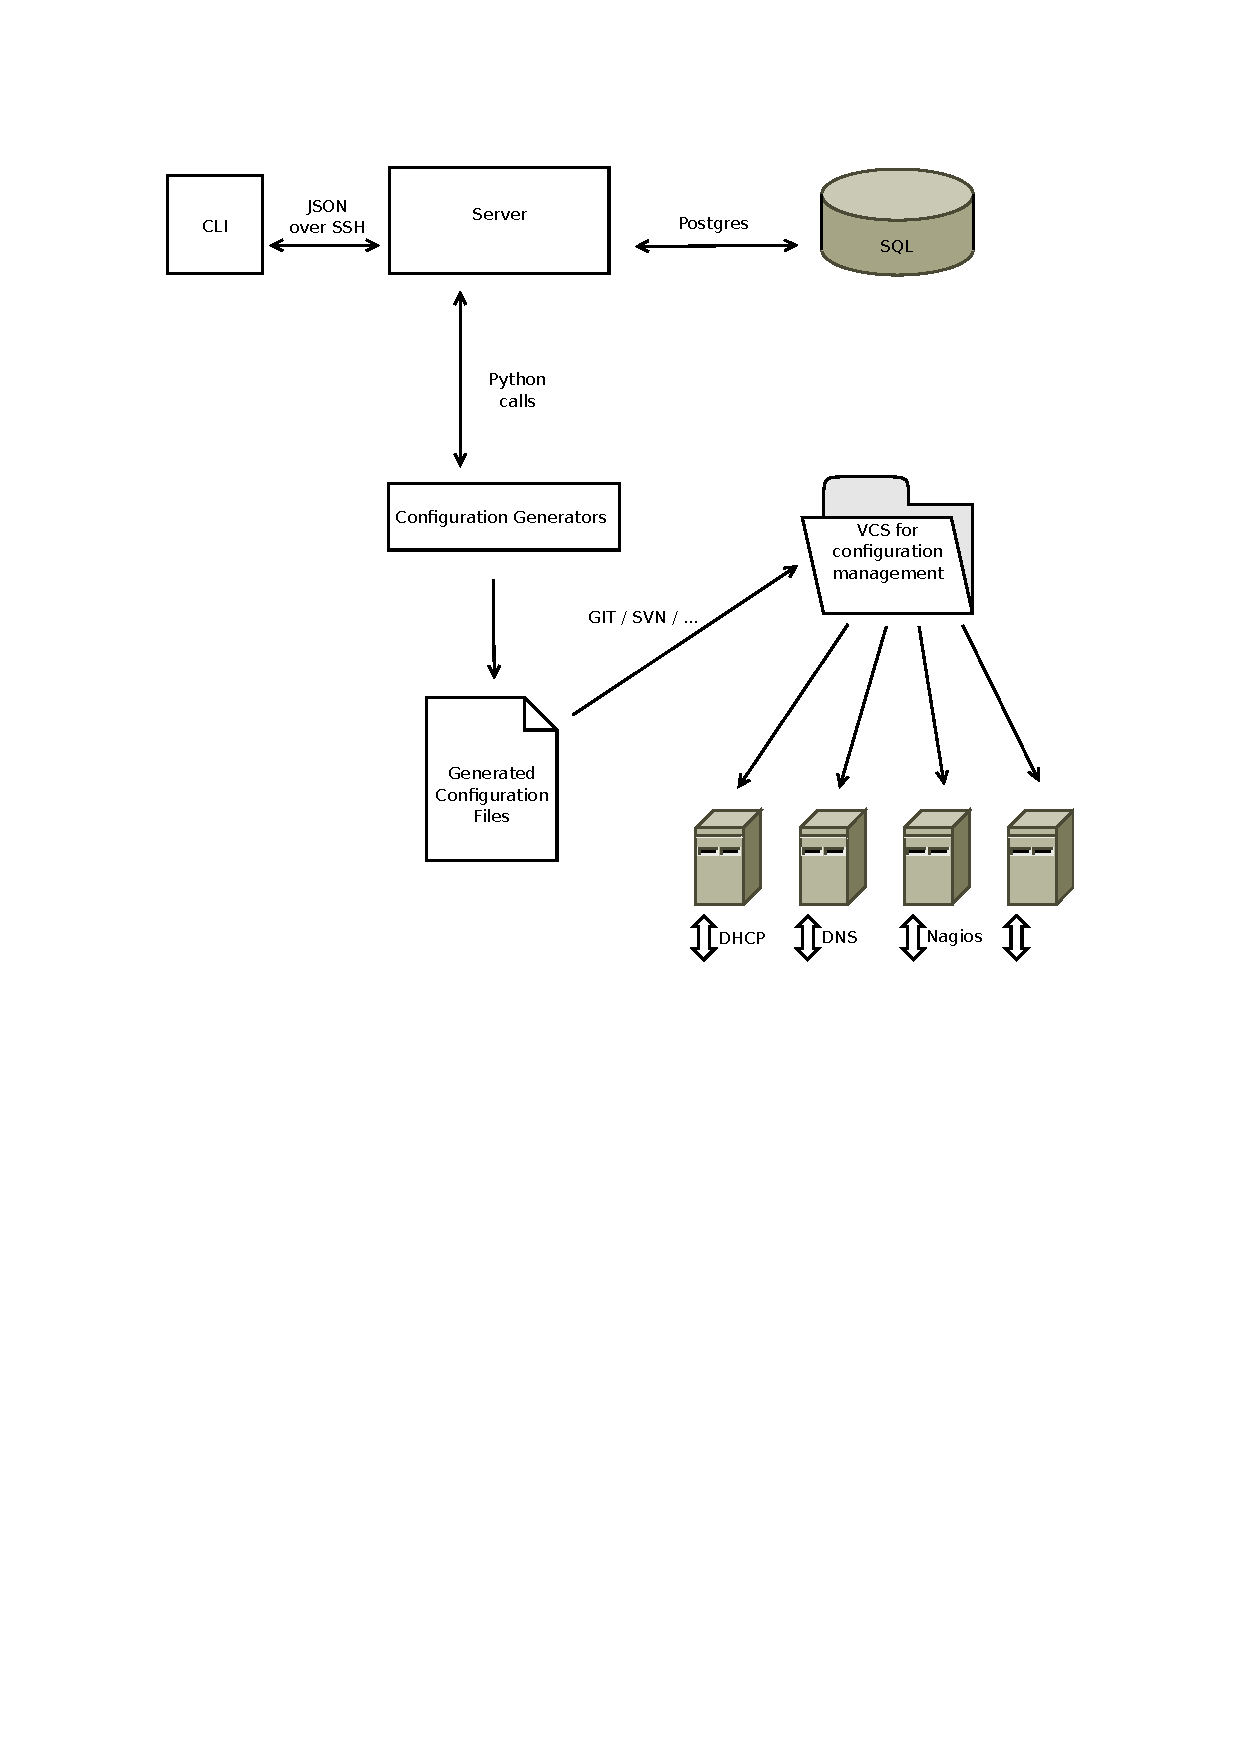
\includegraphics[trim=28mm 134mm 28mm 25mm, clip=true, width=140mm]{img-deska-components.pdf}
    \caption{Structure of a Deska System}
\end{figure}

Second part, the database server, translates the Deska DBAPI commands into calls to stored procedures in the PostgreSQL
server, which in turn performs any required actions.  The database server is implemented in a mixture of PgPython and
PL/PgSQL languages and provides full object-level versioning for all data contained in the Database, with features
similar to Subversion.

The third building block of the Deska system is the scheme definition.  Deska ships with two database schemes, a very
simple one which is intended for testing and demonstration purposes, and another, full-fledged one which suits all needs
of a computing center in Prague.  A database scheme is written in PostgreSQL's native data definition language with full
support for server-side triggers and constraint checks, which are automatically honored by the generated SQL code.

Finally, for the Deska database to actually implement useful functions, a set of scripts is shipped that uses the
information contained in the database and makes it available to various services.  This set of tools is implemented in
pure Python and contains a layer which presents the database contents as a native Python object hierarchy.  This is
further used to create, or {\em generate}, configuration for various services which are in use in Prague, from DHCP
servers and DNS to network switches.  The Deska system, as shipped, comes with everything that is required to plug its
configuration generators to an existing VCS repository of configuration files.

\end{document}
